The direction vector of the line is $\myvec{1 \\ -\sqrt{3}}$. The normal vector $\vec{n}$
\begin{align}
    \vec{n} &= \myvec{0 & -1 \\ 1 & 0}\myvec{1 \\ -\sqrt{3}}\\
    &= \myvec{\sqrt{3} \\ 1}
\end{align}
Let $\vec{P}$ be $\myvec{0 \\ 2}$. The equation of line in terms of normal vector
\begin{align}
    \vec{n}^T(\vec{x} - \vec{P}) &= 0\\
    \implies \myvec{\sqrt{3} & 1}\vec{x} &= \myvec{\sqrt{3} & 1}\vec{P}\\
    \implies \myvec{\sqrt{3} & 1}\vec{x} &= \myvec{\sqrt{3} & 1}\myvec{0 \\ 2}\\
    \implies \myvec{\sqrt{3} & 1}\vec{x} &= 2
\end{align}
The point which crosses the y-axis at a distance of 2 units below the origin
\begin{align}
    \vec{Q} &= \myvec{0 \\ -2}
\end{align}
The equation of line which passes through $\vec{Q}$
\begin{align}
    \vec{n}^T(\vec{x} - \vec{Q}) &= 0\\
    \implies \myvec{\sqrt{3} & 1}\vec{x} &= \myvec{\sqrt{3} & 1}\vec{Q}\\
    \implies \myvec{\sqrt{3} & 1}\vec{x} &= \myvec{\sqrt{3} & 1}\myvec{0 \\ -2}\\
    \implies \myvec{\sqrt{3} & 1}\vec{x} &= -2
\end{align}
    See Fig. \ref{aug/2/20/fig:plot}.
\begin{figure}[htp]
    \centering
    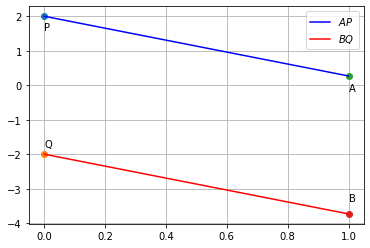
\includegraphics[width=\columnwidth]{solutions/aug/2/20/Figures/Fig1.png}
    \caption{Plot of the given points and lines}
    \label{aug/2/20/fig:plot}
\end{figure}

